\section{Continuous Random Variables}
\subsection{Basic definitions}
Recall that for a probability space $(\Omega,\mathscr F,\mathbb P)$, a random variable is a function $X:\Omega\to\mathbb R$ such that $\{X\le x\}=\{\omega\in\Omega:X(\omega)\le x\}\in\mathscr F$. 

\begin{definition}[Probability distribution function]
    The \textbf{probability distribution function} $ F:\bbR\to [0,1] $ is defined by $F(x)=\mathbb P(X\le x)$.
\end{definition}

\begin{proposition}\
    \begin{enumerate}
        \item $x\le y\implies F(x)\le F(y)$.
        \item $\forall a<b,\mathbb P(a<X\le b)=F(b)-F(a)$.
        \item $F$ is right continuous and the left limits always exist as well. Also,
        $$F(x-)=\mathbb{P}(X<x)\le F(x).$$
        \item $\displaystyle \lim_{x\to-\infty}F(x)=0,\lim_{x\to\infty}F(x)=1.$
    \end{enumerate}
\end{proposition}
\begin{proof}\
    \begin{enumerate}
        \item $ \{X\le x\} \subseteq \{X\le Y\} $.
        \item $ \mathbb{P}(a<x\le b)=\mathbb{P}(\{X>a\}\cap \{X\le b\})=\mathbb{P}(X\le b)-\mathbb{P}(\{X\le b\}\cap \{X\le a\})=\mathbb{P}(X\le b)-\mathbb{P}(X\le a)=F(b)-F(a) $.
        \item It suffices to prove $ \lim_{n \to \infty} F(x+\frac{1}{n})=F(x) $. Define $ A_n=\{x<X\le x+\frac{1}{n}\} $. Then $(A_n)$ are decreasing and $ \cap A_n = \varnothing $. But $ \mathbb{P}(A_n)=F(x+\frac{1}{n})-F(x)\to 0 $, so this proves right continuity. 

        Left limits exist since $F$ is increasing. Note that $ F(x-)=\lim_{n \to \infty} F(x-\frac{1}{n}) $ and that $ F(x-\frac{1}{n})=\mathbb{P}(X\le x-\frac{1}{n}) $. Consider $ B_n=\{X\le x-\frac{1}{n}\} $. Then $ (B_n) \nearrow, \cup B_n=\{X<x\} $, and $ \mathbb{P}(B_n)\to\mathbb{P}(X<x)\to F(x-)\le F(x) $.
        \item This one is easy.
    \end{enumerate}
\end{proof}

For example, $F$ of a discrete random variable might look like this:
\begin{center}
  \begin{tikzpicture}
    \draw [->] (0, 0) -- (3, 0);
    \draw [->] (0, 0) -- (0, 2) node [above] {$F$};
    \draw (0,0.5) -- (1,0.5);
    \node [dot=3.5pt] at (0,0.5) {};
    \draw [dashed] (1,0.5) -- (1,1);
    \node [dot=3.5pt] at (1,1) {};
    \node at (1,0.5) {$ \circ $};
    \draw (1,1) -- (2,1);
    \draw [dashed] (2,1) -- (2,1.5);
    \node [dot=3.5pt] at (2,1.5) {};
    \node at (2,1) {$ \circ $};
    \draw (2,1.5) -- (3,1.5);
    \node at (3,1.5) {$ \circ $};
  \end{tikzpicture}
\end{center}
It is indeed right continuous with left limits.

\begin{definition}[Continuous random variable]
    $X$ is a \textbf{continuous random variable} if $F$ is continuous, which means that $ F(x)=F(x-),\forall x \Longrightarrow \mathbb{P}(X\le x)=\mathbb{P}(X<x),\forall x $. In other words, $ \mathbb{P}(X=x)=0, \forall x\in \mathbb{R}  $.
    \begin{center}
        \begin{tikzpicture}
          \draw [->] (0, 0) -- (3, 0);
          \draw [->] (0, 0) -- (0, 2) node [above] {$F$};
          \draw (0, 0) parabola (2.5, 1.5);
        \end{tikzpicture}
    \end{center}
\end{definition}
\begin{definition}[Absolutely continous]
    $F$ is called \textbf{absolutely continous} if $F$ is not only continuous but also differentiable. 
\end{definition}
In this course we will further restrict to absolutely continuous $F$.

\subsection{Probability density function}

\begin{definition}[Probability density function]
    Set $F'(x)=f(x)$. We call $f$ the \textbf{probability density function} of $X$. 
\end{definition}

\begin{proposition}[Properties of $f$]\
    \begin{enumerate}
        \item$f(x)\ge 0$.
        \item $ \int_{-\infty}^x f(y)\,\mathrm dy=F(x). $ In particular, $ \int_{-\infty}^\infty f(y)\,\mathrm dy=1. $
    \end{enumerate}
\end{proposition}
Intuitively, for $\Delta x$ small, we have
\[
    \mathbb P(x<X\le x+\Delta x)=\int_x^{x+\Delta x}f(y)\,\mathrm dy\approx f(x)\Delta x,
\]
which is like approximating a continuous random variable by the probability density function of a discrete random variable. 

More generally, for any set $ S \subseteq \mathbb{R}  $, 
\[
    \mathbb{P}(x\in S) = \int_{S} f(x) \,\mathrm{d}x.
\]

\begin{center}
    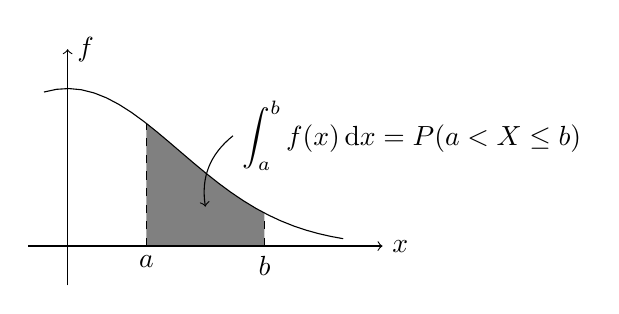
\begin{tikzpicture}
        \fill [gray, domain=1:2.5, variable=\x]
        (1, 0)
        -- plot (\x, {2 * exp(-\x * \x / 4)})
        -- (2.5, 0)
        -- cycle;
        \draw [->] (-0.5,0) -- (4,0) node [right] {$ x $};
        \draw [->] (0,-0.5) -- (0,2.5) node [right] {$ f $};
        \draw [domain=-0.3:3.5, variable=\x] plot (\x, {2 * exp(-\x * \x / 4)});
        \node [below] at (1,0) {$a$};
        \node [below] at (2.5,0) {$b$};
        \draw [->, bend right] (2.1, 1.4) to (1.75, 0.5);
        \node [right] at (2.1, 1.4) {$\displaystyle \int_{a}^{b} f(x) \,\mathrm{d}x = \mathbb{P}(a<X\le b)$};
        \draw [dashed] (1,0) -- (1,1.56);
        \draw [dashed] (2.5,0) -- (2.5,0.42);
    \end{tikzpicture}
\end{center}

\subsection{Expectation and variance}
\begin{definition}[Expectation of positive continuous r.v.]
    Let $X\ge 0$ with density $f$. Define its \textbf{expectation} as 
    \[
        \bbE[X] = \int_{0}^{\infty} xf(x) \,\mathrm{d}x.
    \]
\end{definition}\
\begin{note}
    Suppose $g\ge 0$. Then for any variable $X$,
    \[
        \bbE[g(X)]= \int_{-\infty}^{\infty} g(x)f(x) \,\mathrm{d}x.
    \]
\end{note}
\begin{definition}[Expectation of general continuous r.v.]
    Let $X$ be a general r.v. Define $ X_+=\max \{X,0\},X_-=\max \{-X,0\} $. If at least one of $ \bbE[X_+],\bbE[X_-] $ is finite, then define 
    \[
        \bbE[X]=\bbE[X_+]-\bbE[X_-] = \int_{-\infty}^{\infty} xf(x) \,\mathrm{d}x.
    \]
\end{definition}
\begin{note}
    The last equality comes from 
    \[
        \bbE[X_+] = \int_{0}^{\infty} xf(x) \,\mathrm{d}x,\quad \bbE[X_-]=\int_{-\infty}^{0} xf(x) \,\mathrm{d}x.
    \]
    It is easy to check that the expectation is a \textit{linear} function.
\end{note}

\begin{proposition}
    Let $X\ge 0$. Then 
    \[
        \bbE[X] = \int_{0}^{\infty} \mathbb{P}(X\ge x) \,\mathrm{d}x.
    \]
\end{proposition}
\begin{proof}
    \begin{align*}
        \bbE[X]&= \int_{0}^{\infty} xf(x) \,\mathrm{d}x=\int_{0}^{\infty} \left( \int_{0}^{x}  \,\mathrm{d}y \right)f(x) \,\mathrm{d}x\\ 
        \text{(Check!)}&= \int_{0}^{\infty} \int_{y}^{\infty} f(x) \,\mathrm{d}x \,\mathrm{d}y = \int_{0}^{\infty} (1-F(y)) \,\mathrm{d}y\\ 
        &= \int_{0}^{\infty} \mathbb{P}(X\ge y) \,\mathrm{d}y.\qedhere
    \end{align*}
\end{proof}
\begin{proof}[Alternatively,]
    note that $ \forall \omega, X(\omega)=\int_{0}^{\infty} 1(X(\omega)\ge x) \,\mathrm{d}x $. Taking expectation we get 
    \begin{align*}
        \bbE[X] &= \bbE\left[ \sum_{\omega}\int_{0}^{\infty} 1(X(\omega)\ge x) \,\mathrm{d}x \right] = \bbE\left[ \int_{0}^{\infty} 1(X\ge x) \,\mathrm{d}x \right]\\
        &= \int_{0}^{\infty} \bbE[1(X(\omega)\ge x)] \,\mathrm{d}x = \int_{0}^{\infty} \mathbb{P}(X\ge x) \,\mathrm{d}x.\qedhere
    \end{align*}
\end{proof}
\begin{remark}
    The second proof is not rigorous since we did not justify interchanging $ \bbE $ and $ \int $.
\end{remark}

\begin{definition}[Variance]
    The \textbf{variance} of a continuous random variable is
    \[
        \var(X) = \bbE[(X-\bbE[X])^2] = \bbE[X^2]-(\bbE[X])^2.
    \]
\end{definition}

\subsection{Examples of continuous r.v.s}
\begin{example}[Uniform distribution]
    Let $a,b\in \bbR$ such that $a<b$. Define the density as 
\[
    f(x) = \begin{cases}
    \frac{1}{b-a} &\text{if }x\in [a,b]\\
    0 &\text{otherwise}\\
    \end{cases} 
\]
Then $X$ is called a \textbf{uniform} distribution and we write $ X \sim U[a,b] $, and the pdf is 
\[
    F(x)=\mathbb P(X\le x)=\int_{-\infty}^xf(y)\,\mathrm dy=\begin{cases}
        0&\text{if $x<a$}\\
        \frac{x-a}{b-a}&\text{if $x\in [a,b]$}\\
        1&\text{if $x>b$}
    \end{cases},
\]
and $ \bbE[X] $ is 
\[
    \mathbb E[X]=\int_{-\infty }^{\infty }xf(x)\,\mathrm dx=\int_a^bxf(x)\,\mathrm dx=\frac{a+b}{2}
\]
\end{example}

\begin{example}[Exponential distribution]
    The density is $ f(x)=\lambda e^{-\lambda x} $ where $ \lambda,x>0 $. Write $ X \sim \operatorname{Exp}(\lambda) $. Here 
    \[
        F(x)=\int_0^x\lambda e^{-\lambda y}\,\mathrm dy=1-e^{-\lambda x},.\quad \bbE[X]=\int_{0}^{\infty} \lambda x e^{-\lambda x} \,\mathrm{d}x=\frac{1}{\lambda}.
    \]
    \paragraph{Exponential as a limit of geometrics.} Let $T\sim\operatorname{Exp}(\lambda)$ and $T_n=\lfloor nT\rfloor$, so
    \[
        \mathbb P(T_n\ge k)=\mathbb P(T\ge k/n)=e^{-k\lambda/n}=(e^{-\lambda/n})^k,
    \]
    so $T_n$ is distributed geometrically with parameter $p_n=1-e^{-\lambda/n}$, so as $n\to\infty$, we have $p_n\sim \lambda/n$ and $T_n/n\to T$. So exponential is the limit of a rescaled geometric.
\end{example}

\begin{proposition}
    The exponential random variable is \emph{memoryless}, i.e.
    \[
        \bbP(T > t+s \mid T>s) = \bbP(T>t).
    \]
\end{proposition}
We have something stronger:
\begin{proposition}
    Let $ T $ be a positive continous r.v. not identically $0$ or $ \infty $ with density $f$. Then $T$ is memoryless if and only if $T$ is exponential.
\end{proposition}
\begin{proof}
    $ (\Leftarrow) $ is justified by proposition 3.4. $ (\Rightarrow ) $: Suppose $ \forall s,t,\ \mathbb{P}(T>t+s)=\mathbb{P}(T>s)\mathbb{P}(T>t) $. Set $ g(t)=\mathbb{P}(T>t) $. We want to show $ g(t)=e^{-\lambda t} $ for some $ \lambda>0 $. Note that $ \forall s,t>0,\ g(t+s)=g(t)g(s) $, and 
    \[
        \forall t\ge 0, \forall m\in \mathbb{N},\ g(mt)=(g(t))^m \Longrightarrow g(m)=g(1)^m.
    \]
    Furthermore, 
    \[
        \forall m,n\in \mathbb{N},\ g\left( \frac{m}{n} \right)^n=g(m) \Longrightarrow g\left( \frac{m}{n} \right)= g(m)^{1/n}=g(1)^{m/n}.
    \]
    Now $ g(1)=\mathbb{P}(T>1)\in (0,1) $, as $T$ would be identically $0$ or $ \infty $ otherwise. Set $ \lambda=-\log \mathbb{P}(T>1)>0 $. So we have proved that 
    \[
        \forall t\in \mathbb{Q}_+,\ g(t)=\mathbb{P}(T>t)=e^{-\lambda t}.
    \]
    Let $ t\in \mathbb{R}_+ $. Then $ \forall \epsilon,\ \exists r,s\in \mathbb{Q} $ such that $ r\le t\le s $ and $ |r-s|<\epsilon $. Now
    \[
        e^{-\lambda s}=\mathbb{P}(T>s)\le \mathbb{P}(T>t)\le \mathbb{P}(T>r) = e^{-\lambda r}.
    \]
    Since it holds for all $ \epsilon $, we must have $ \mathbb{P}(T>t)=e^{-\lambda t} $, as claimed.
\end{proof}

\begin{theorem}\label{thm:3.6}
    Let $X$ be a continuous random variable with density $f$.
    Let $g$ be a continuous, strictly monotone function with $g^{-1}$ differentiable.
    Then $g(X)$ is a continuous random variable with density
    \[
        f(g^{-1}(x))\left| \frac{\mathrm{d}}{\mathrm{d}x}g^{-1}(x) \right|. 
    \]
\end{theorem}
\begin{proof}
    First assume that $g$ is strictly increasing, then $\mathbb P(g(X)\le x)=\mathbb P(X\le g^{-1}(x))=F(g^{-1}(x))$, so the density of $g(X)$ would be
    $$\frac{\mathrm d}{\mathrm dx}F(g^{-1}(x))=f(g^{-1}(x))\frac{\mathrm dg^{-1}(x)}{\mathrm dx}=f(g^{-1}(x))\left|\frac{\mathrm dg^{-1}(x)}{\mathrm dx}\right|.$$
    As for $g$ strictly decreasing, $\mathbb P(g(X)\le x)=\mathbb P(X\ge g^{-1}(x))=1-F(g^{-1}(x))$, so the density is
    $$\frac{\mathrm d}{\mathrm dx}(1-F(g^{-1}(x)))=-f(g^{-1}(x))\frac{\mathrm dg^{-1}(x)}{\mathrm dx}=f(g^{-1}(x))\left|\frac{\mathrm dg^{-1}(x)}{\mathrm dx}\right|,$$
    as claimed.
\end{proof}
\begin{example}[Normal distribution]
    For $\mu\in\mathbb R,\sigma>0$, define $ f: \mathbb{R}\to \mathbb{R} $ by
    \[
        f(x) = \frac{1}{\sqrt{2\pi\sigma^2}}\exp\left(-\frac{(x - \mu)^2}{2\sigma^2}\right).
    \]
    \begin{center}
        \begin{tikzpicture}[yscale=1.5]
          \draw (-3, 0) -- (3, 0);
          \draw (0, 1.3) -- (0, 0) node [below] {$\mu$};
          \draw [domain=-3:3,samples=50, blue] plot (\x, {exp(-\x * \x)});
        \end{tikzpicture}
    \end{center}
    \begin{proof}[Check that $f$ is a density]
        Indeed, 
        \begin{align*}
            \int_{-\infty}^{\infty} f(x) \,\mathrm{d}x &= \int_{-\infty}^{\infty} \frac{1}{\sqrt{2\pi\sigma^2}}\exp\left(-\frac{(x - \mu)^2}{2\sigma^2}\right) \,\mathrm{d}x\\ 
            &= \int_{-\infty}^{\infty} \frac{1}{\sqrt{2\pi}}\exp \left( -\frac{u^2}{2} \right)\dd u\\ 
            &= 2 \int_{0}^{\infty} \frac{1}{\sqrt{2\pi}} \exp \left( -\frac{u^2}{2} \right)\dd u=:I.
        \end{align*}
        Then
        \begin{align*}
          I^2 &= \frac{\pi}{2} \int_{0}^{\infty} \int_{0}^{\infty} \exp \left( -\frac{u^2+v^2}{2} \right) \,\mathrm{d}u\,\mathrm{d}v\\ 
          &= \frac{\pi}{2}\int_0^\infty \int_0^{\pi/2}re^{-r^2/2}\dd r\dd \theta=1\\ 
          \Longrightarrow I&=1.\qedhere
        \end{align*}
    \end{proof}
    \begin{proposition}
        $\bbE[X] = \mu$.
    \end{proposition}
    \begin{proof}
    \begin{align*}
    \bbE[X] &= \frac{1}{\sqrt{2\pi}\sigma} \int_{-\infty}^\infty x e^{-(x - \mu)^2/2\sigma^2}\dd x\\
    &= \frac{1}{\sqrt{2\pi} \sigma}\int_{-\infty}^\infty (x - \mu)e^{-(x - \mu)^2/2\sigma^2}\dd x + \frac{1}{\sqrt{2\pi}\sigma}\int_{-\infty}^\infty \mu e^{-(x - \mu)^2/2\sigma^2}\dd x.
    \end{align*}
    The first term is antisymmetric about $\mu$ and gives $0$. The second is just $\mu$ times the integral we did above. So we get $\mu$.
    \end{proof}
    \begin{proposition}
    $\var(X) = \sigma^2$.
    \end{proposition}
    \begin{proof}
    We have $\var (X) = \bbE[X^2] - (\bbE[X])^2$. Substitute $Z = \frac{X - \mu}{\sigma}$. Then $\bbE[Z] = 0$, $\bbE[Z^2] = \frac{1}{\sigma^2}\bbE[X^2]$. Then
    \begin{align*}
        \var(Z) &= \frac{1}{\sqrt{2\pi}} \int_{-\infty}^\infty z^2 e^{-z^2/2}\dd z\\
        &= \left[-\frac{1}{\sqrt{2\pi}}ze^{-z^2/2}\right]_{-\infty}^\infty + \frac{1}{\sqrt{2\pi}}\int_{-\infty}^\infty e^{-z^2/2}\dd z\\
        &= 0 + 1\\
        &= 1
    \end{align*}
    So $\var X = \sigma^2$.
    \end{proof}
    When $X$ has density $ f $, $X$ has the \textbf{normal distribution} and we write $ X \sim \mcN(\mu,\sigma^2) $. So the distribution and density of the standard normal $ \mcN(0,1) $ is
    \[
        \Phi(x)=\int_{-\infty}^x\frac{e^{-t^2/2}}{\sqrt{2\pi}}\,\mathrm dt,\quad\phi(x)=\Phi'(x)=\frac{e^{-x^2/2}}{\sqrt{2\pi}}.
    \]
    Since $ \phi(x)=\phi(-x) \Rightarrow \Phi(x)+\Phi(-x)=1 $, we have 
    \[
        \mathbb{P}(X\le x)=1-\mathbb{P}(X\le -x).
    \]
\end{example}

\begin{example}[Composition of normal distributions]
    Let $ X \sim \mcN( \mu,\sigma^2) $. Let $ a,b\in \mathbb{R} $ such that $ a\neq 0 $. Set $ g(x)=ax+b $ and define 
    \[
        Y= g(X).
    \]
    What is the density of $Y$?

    Note that $g$ is strictly monotone and $ g^{-1}(x)=\frac{x-b}{a} $ is differentiable. Hence by theorem \ref{thm:3.6}, the density of $y$ is 
    \begin{align*}
        f_Y(y)&= f_X(g^{-1}(y)) \left| \frac{\mathrm{d}}{\mathrm{d}y} g^{-1}(y)  \right| \\ 
        &= \frac{1}{\sqrt{2\pi\sigma^2}}\exp\left(-\frac{(\frac{y-b}{a} - \mu)^2}{2\sigma^2}\right) \frac{1}{|a|}\\ 
        &= \frac{1}{\sqrt{2\pi a^2\sigma^2}} \exp \left( -\frac{(y-b - a\mu)^2}{2a^2\sigma^2} \right).
    \end{align*}
    So 
    \[
        Y \sim \mcN\left( a\mu+b, a^2\sigma ^2 \right).
    \]
    The importance here is that 
    \[
        \boxed{X \sim \mcN(\mu,\sigma^2) \Longrightarrow \frac{X-\mu}{\sigma}\sim \mcN(0,1)}
    \]
    Notice that 
    \[
        \mathbb{P}(-2\sigma<X-\mu<2\sigma)=\mathbb{P}\left( -2<\frac{X-\mu}{\sigma}<2 \right)=\Phi(2)-\Phi(-2)\ge 0.95,
    \]
    so 
    \begin{quote}
        \textit{With probability $ 95\% $ the normal is within 2 standard deviations of the mean.}
    \end{quote}
\end{example}
\subsection{Median and mode}
\begin{definition}
    Suppose $X$ is a continous r.v. The \textbf{median} of $X$, $m$, is the number satisfying 
    \[
        \mathbb{P}(X\le m)=\mathbb{P}(X\ge m)=\frac{1}{2}.
    \]
    In other words,
    \[
        \int_{-\infty}^{m} f(x) \,\mathrm{d}x=\int_{m}^{\infty} f(x) \,\mathrm{d}x = \frac{1}{2}.
    \]
\end{definition}
\begin{example}[Median of normal]
    Let $ X \sim \mcN(\mu,\sigma^2) $. Check that $ m=\mu $.
\end{example}
\begin{definition}[Mode]
    Given a pdf $f(x)$, we call $\hat x$ a \textbf{mode} if
    \[
        f(\hat x) \geq f(x)
    \]
    for all $x$. Note that a distribution can have many modes. For example, in the uniform distribution, all $x$ are modes.
\end{definition}
\subsection{Multivariate density functions}
\begin{definition}
    Let $ \bfX = (X_1,\dots,X_n)\in \mathbb{R}^{n} $ be a r.v. We say that $\bfX$ has density $f$ if 
    \begin{align*}
        F(x_1,\dots,x_n) &= \mathbb{P}(X_1\le x_1,\dots X_n\le x_n)\\ &= \int_{-\infty}^{x_n} \cdots \int_{-\infty}^{x_1} f(y_1,\dots,y_n)\dd y_1\cdots\dd y_n.
    \end{align*}
\end{definition}
\begin{note}
    Then 
    \[
        f(x_1,\dots,x_n) = \frac{\partial^n }{\partial x_1 \cdots \partial x_n}F(x_1,\dots,x_n). 
    \]
    We can generalise to any\footnote{Not quite. See II Probability and Measure.} $ B \subseteq \mathbb{R}^{n} $: 
    \[
        \mathbb{P}(\bfX\in B) = \int_B f(y_1,\dots,y_n)\dd y_1\cdots\dd y_n.
    \]
\end{note}
\begin{definition}[Independence]
    We say $X_1,\dots,X_n$ are \textbf{independent} if $ \forall x_1,\dots,x_n\in \mathbb{R} $, 
    \[
        \mathbb{P}(X_1\le x_1,\dots, X_n\le x_n) = \mathbb{P}(X_1\le x_1)\cdots \mathbb{P}(X_n\le x_n).
    \]
\end{definition}
\begin{theorem}\label{thm:3.9}
    Let $ \bfX = (X_1,\dots,X_n) $ have density $f$.
    \begin{enumerate}
        \item If $ X_1,\dots,X_n $ are independent with densities $ f_i $, then 
        \[
            f(x_1,\dots,x_n)=f_1(x_1) \cdots f_n(x_n).
        \]
        \item If $f$ factorises to the above equation, then $ X_1,\dots,X_n $ are independent with densities proportional to $ f_i $.
    \end{enumerate}
\end{theorem}
\begin{proof}
    \begin{enumerate}
        \item Suppose $ X_1,\dots,X_n $ are independent with densities $ f_i $. By definition, 
        \begin{align*}
            &\mathbb{P}(X_1\le x_1,\dots, X_n\le x_n) = \mathbb{P}(X_1\le x_1)\cdots \mathbb{P}(X_n\le x_n)\\ 
            =& \prod_{i=1}^{n} \int_{-\infty}^{x_i} f_i(y_i) \,\mathrm{d}y_i
            = \int_{-\infty}^{x_n} \cdots \int_{-\infty}^{x_1} \prod_{i=1}^{n}f_i(y_i)\dd y_1\cdots\dd y_n.\ 
        \end{align*}
        Hence the density of $\bfX$ is $\prod f_i $.
        \item By assumption, if $ B_i\in \mathbb{R}, $ then 
        \[
            \mathbb{P}(X_i\in B_i) = \int_{B_n} \cdots \int_{B_1} \prod_{i=1}^{n}f_i(y_i) \,\mathrm{d}y_1\cdots \,\mathrm{d}y_n.
        \]
        Let $ B_j=\mathbb{R}, j\neq i $, then 
        \[
            \mathbb{P}(X_i\in B_i)= \int_{B_i} f_i(y_i) \,\mathrm{d}y_i \prod_{j\neq i} \int_{\bbR} f_j(y_j) \,\mathrm{d}y_j.
        \]
        Note that 
        \[
            \prod_{i=1}^{n}\int_{\bbR} f_i(y_i) \,\mathrm{d}y_i=1,
        \]
        so we have 
        \[
            \mathbb{P}(X_i\in B_i) = \frac{\int_{B_i} f_i(y_i) \,\mathrm{d}y_i}{\int_{\bbR} f_i(y_i) \,\mathrm{d}y_i},
        \]
        and the density of $X_i$ is 
        \[
            \frac{f_i}{\int_{\bbR} f_i(y_i) \,\mathrm{d}y_i}.
        \]
        To check $X_i$ are independent, note that 
        \begin{align*}
            \mathbb{P}(X_i\le x_i)&= \frac{\int_{-\infty}^{x_1} f_1(y_1) \,\mathrm{d}y_1 \cdots \int_{-\infty}^{x_n} f_n(y_n) \,\mathrm{d}y_n}{\int_{\bbR} f_1(y_1) \,\mathrm{d}y_1 \cdots \int_{\bbR} f_n(y_n) \,\mathrm{d}y_n}\\ 
            &= \mathbb{P}(X_1\le x_1)\cdots \mathbb{P}(X_n\le x_n).\qedhere
        \end{align*}
    \end{enumerate}
\end{proof}

Suppose $ (X_1,\dots,X_n) $ has density $f$. Then 
\begin{align*}
    \mathbb{P}(X_1\le x)&= \mathbb{P}(X_1\le x,X_2\in \mathbb{R}, \dots, X_n \in \mathbb{R})\\ 
    &= \int_{\bbR} \cdots \int_{-\infty}^{x} f(x_1,\dots,x_n) \,\mathrm{d}x_1 \, \cdots \mathrm{d}x_n\\ 
    &= \int_{-\infty}^{x} \left( \int_{\bbR}\cdots \int_{\bbR} f(x_1,\dots,x_n) \,\mathrm{d}x_2 \,\cdots\mathrm{d}x_n \right) \,\mathrm{d}x_1.
\end{align*}
\begin{definition}
    The \textbf{marginal density} of $X_1$ is defined by 
    \[
        f_{X_1}(x) = \int_{\bbR}\cdots \int_{\bbR} f(x_1,\dots,x_n) \,\mathrm{d}x_2\cdots \,\mathrm{d}x_n.
    \]
\end{definition}
\subsection{Density of the sum of independent r.v.s}
\begin{proposition}\label{prop:3.10}
    Suppose $ X,Y $ are independent r.v.s with densities $ f_X,f_Y $. Then the density of $ X+Y $ is 
    \[
        \int_\bbR f_Y(y-x)f_X(x)\dd x .
    \]
\end{proposition}
\begin{proof}
    Let $A=\{x+y\le z\}$.
    \begin{align*}
        \mathbb{P}(X+Y\le z)&=\iint_A f_{X,Y}(x,y)\dd x\dd y\\ 
        &= \int_{-\infty}^{z-x} \,\mathrm{d}y \int_{\bbR} \,\mathrm{d}x\ f_X(x)f_Y(y)\\ 
        &= \int_{\bbR} \,\mathrm{d}x \int_{-\infty}^{z} \,\mathrm{d}y\ f_X(x)f_Y(y-x)\\ 
        &= \int_{-\infty}^{z} \,\mathrm{d}y \left( \int_{\bbR} f_X(x)f_Y(y-x)\,\mathrm{d}x \right).\qedhere
    \end{align*}
\end{proof}

\begin{definition}
    For 2 densities $f,g$, the \textbf{convolution} of $f,g$ is 
    \[
        \int_\bbR f(x-y)g(y)\dd y.
    \]
\end{definition}

\subsection{Conditional density and expectation}
\begin{definition}
    Let $X$ and $Y$ be continous r.v.s with joint density $ f_{X,Y} $ and marginal densities $ f_X,f_Y $. The \textbf{conditional density} of $X$ given $ Y=y $ is defined as 
    \[
        f_{X|Y}(x|y) = \frac{f_{X,Y}(x,y)}{f_Y(y)}.
    \]
\end{definition}
\begin{proposition}[Law of total probability]
    \[
        f_X(x) = \int_{-\infty}^{\infty} f_{X|Y}(x|y)f_Y(y) \,\mathrm{d}y.
    \]
\end{proposition}
\begin{proof}
    $ f_X(x) = \int_{-\infty}^{\infty} f_{X,Y}(x,y) \,\mathrm{d}y = \int_{-\infty}^{\infty} f_{X|Y}(x|y)f_Y(y) \,\mathrm{d}y. $
\end{proof}

\begin{definition}
    Let 
    \[
        g(y)=\int_{-\infty}^{\infty} xf_{X|Y}(x|y) \,\mathrm{d}x,
    \]
    define the \textbf{conditional expectation} as $ \bbE[X|Y]=g(Y) $.
\end{definition}

\subsection{Transformation of multidimensional r.v.s}
\begin{theorem}
    Let $\bfX$ be a r.v. with values in $ D \subseteq \mathbb{R}^{d} $ with density $ f_\bfX: \mathbb{R}^{d}\to \mathbb{R} $. Let $\bfg: \mathbb{R}^{d}\to \mathbb{R}^{d}$ be a bijection $ D \to \bfg(D) $ that has a continous derivative on $D$ and $ \det \bfg'(\bfx)\neq 0,\ \forall \bfx\in D $. Then the r.v. $ \bfY=\bfg(\bfX) $ has density 
    \[
        f_\bfY(\bfy) = f_\bfX(\bfx) \cdot |J|,
    \]
    where $ \bfx=\bfg^{-1}(\bfy) $ and $J$ is the Jacobian of $ \bfx,\bfy $:
    \[
        J = \frac{\partial (x_1,\dots,x_d)}{\partial (y_1,\dots, y_d)}.
    \]
\end{theorem}
\begin{proof}
    Search Wikipedia or something.
\end{proof}

\begin{example}
    Let $ X,Y $ be independent $ \mcN(0,1) $ r.v.s. What is the density of $ (R,\Theta) $, where $ R=\sqrt{X^2+Y^2} $ and $ \Theta = \arctan (Y/X) $?
    \begin{center}
        \begin{tikzpicture}
            \draw (-0.5,0) -- (2,0);
            \draw (0,-0.5) -- (0,2);
            \draw [blue] (0,0) -- (1,1.732) node [dot=3pt] {} node [pos=0.5,above left] {{\color{red}$ R $}};
            \node [above right] at (1,1.732) {$ (X,Y) $};
            \centerarc[red](0,0)(0:60:0.3);
            \node at (0.26,0.1) [above right] {{\color{red}$ \Theta $}};
        \end{tikzpicture}
    \end{center}
    Clearly $ X=R \cos \Theta,Y=R \sin \Theta $, so by theorem 
    \[
        f_{R,\Theta}(r,\theta) = f_{X,Y}(r \cos \theta,r \sin \theta)|J|=rf_{X,Y}(r \cos \theta,r \sin \theta).
    \]
    By independence of $ X,Y $, can check that 
    \[
        f_{R,\Theta}(r,\theta) = \frac{1}{2\pi}re^{-r^2/2},\quad r>0, \theta\in [0,2\pi].
    \]
    Hence $R \independent \Theta$ and $ f_R=re^{-r^2/2},\ f_\Theta=1/2\pi $, i.e. $ \Theta \sim U[0,2\pi] $.
\end{example}
\subsection{Order statistics for random samples}
\begin{definition}
    Let $ X_1,\dots,X_n $ are iid rvs with distribution $ F $ and density $f$. Let $Y_1, \cdots, Y_n$ be $X_1, \cdots, X_n$ arranged in increasing order, i.e.\ $Y_1 \le Y_2 \le \cdots \le Y_n$. This is the \textbf{order statistics}.
\end{definition}
Immediately we get 
\begin{align*}
    \mathbb P(Y_1\le x)&=1-\mathbb P(Y_1>x)=1-(1-F(x))^n,\\ 
    f_{Y_1}(x)&= nf(x)(1-F(x))^{n-1},\\
    \mathbb P(Y_n\le x)&=(F(x))^n,\\ 
    f_{Y_n}(x)&=nf(x)F(x)^{n-1}.
\end{align*}
\begin{proposition}
    The joint density of $(Y_1,\ldots,Y_n)$ is given by 
    \[
        f_{Y_1,\dots,Y_n}(x_1,\ldots,x_n) = \begin{cases}
            n!f(x_1)\cdots f(x_n) &\text{if } x_1<\cdots<x_n,\\
         0&\text{otherwise}.\\
        \end{cases} 
    \]
\end{proposition}
\begin{proof}
    Let $x_1<\cdots<x_n$, we have
    \begin{align*}
        \mathbb P(Y_1\le x_1,\ldots,Y_n\le x_n)&=\sum_{\sigma\in S_n}\mathbb P(X_1\le x_{\sigma(1)},\ldots X_n\le x_{\sigma(n)})\\
        &=n!\mathbb P(X_1\le x_1,\ldots X_n\le x_n)\\
        &=n!\int_{-\infty}^{x_1}f(u_1)\int_{-\infty}^{x_2}f(u_2)\cdots\int_{-\infty}^{x_n}f(u_n)\,\mathrm du_n\cdots\mathrm  du_1.
    \end{align*}
    Differentiating gives the result.
\end{proof}
\begin{example}
    Let $ X \sim \operatorname{Exp}(\lambda),Y \sim \operatorname{Exp}(\mu) $ be independent r.v.s and let $ Z=\min (X,Y) $. i.e. let $X,Y$ denote 2 clocks whose distributions of rings are exponentials with parameters $ \lambda,\mu $, so $Z$ is the first ring. Then 
    \[
        \mathbb{P}(Z\ge z) = \mathbb{P}(X\ge z,Y\ge z) = e^{-(\lambda+\mu)z},
    \]
    so $ Z \sim \operatorname{Exp} (\lambda+\mu) $. More generally, if $ X_1,\dots,X_n $ are independent with $ X_i \sim \operatorname{Exp}(\lambda_i) $, then 
    \[
        \min (X_1,\dots,X_n) \sim \operatorname{Exp}\left( \sum_{i=1}^{n}\lambda_i \right).
    \]
\end{example}
\begin{example}
    Let $X_1,\ldots,X_n$ be iid $\operatorname{Exp}(\lambda)$ and $Y_i$ be the order statistics and $Z_1=Y_1,Z_i=Z_i-Z_{i-1}$ for $i=2,\ldots,n$.
    i.e. let $X_1,\dots,X_n$ be $n$ clocks, $Y_i$ are ordered according to which rings first. Then $Z_1$ is the first ring, and $ Z_i $ are times between $ Z_i $ and $ Z_{i-1} $.

    Then
    $$\bfZ=\begin{pmatrix}
        Z_1\\
        \vdots\\
        Z_n
    \end{pmatrix}=A\begin{pmatrix}
        Y_1\\
        \vdots\\
        Y_n
    \end{pmatrix},A=\begin{pmatrix}
        1&0&0&\cdots&0\\
        -1&1&0&\cdots&0\\
        0&-1&1&\cdots&0\\
        \vdots&\vdots&\vdots&\ddots&\vdots\\
        0&0&0&\cdots&1
    \end{pmatrix}$$
    where we have $\det A=1$ and $Y_j=\sum_{i=1}^jZ_i$, so for $y_j=\sum_{i=1}^jz_i$, we have
    \begin{align*}
        f_{Z_1,\ldots,Z_n}(z_1,\ldots,z_n)&=f_{Y_1,\ldots,Y_n}(y_1,\ldots,y_n)|J|\\
        &=n!e^{-\lambda y_1}\cdots e^{-\lambda y_n}\\
        &=n!\lambda^ne^{-\lambda(nz_1+(n-1)z_2+\cdots +2z_{n-1}+z_n)}\\
        &=\prod_{i=1}^n(n-i+1)\lambda e^{-\lambda(n-i+1)z_1}.
    \end{align*}
    So $(Z_1,\ldots,Z_n)$ are independent exponentials with $Z_i\sim\operatorname{Exp}(\lambda(n-i+1))$.
\end{example}